%% LyX 2.0.3 created this file.  For more info, see http://www.lyx.org/.
%% Do not edit unless you really know what you are doing.
\documentclass[12pt,english]{report}
\usepackage[T1]{fontenc}
\usepackage[latin9]{inputenc}
\usepackage{float}
\usepackage{calc}
\usepackage{amsthm}
\usepackage{amsmath}
\usepackage{setspace}

\makeatletter

%%%%%%%%%%%%%%%%%%%%%%%%%%%%%% LyX specific LaTeX commands.
\providecommand{\LyX}{L\kern-.1667em\lower.25em\hbox{Y}\kern-.125emX\@}
%% Because html converters don't know tabularnewline
\providecommand{\tabularnewline}{\\}
\floatstyle{ruled}
\newfloat{algorithm}{tbp}{loa}[chapter]
\providecommand{\algorithmname}{Algorithm}
\floatname{algorithm}{\protect\algorithmname}

%%%%%%%%%%%%%%%%%%%%%%%%%%%%%% Textclass specific LaTeX commands.
\usepackage{UTSAthesis}      
\usepackage{times}            
\usepackage{latexsym}

\newenvironment{ruledcenter}{%
  \begin{center}
  \rule{\textwidth}{1mm} } {%
  \rule{\textwidth}{1mm} 
  \end{center}}%


  \theoremstyle{definition}
  \newtheorem{defn}{\protect\definitionname}
\theoremstyle{plain}
\newtheorem{thm}{\protect\theoremname}

%%%%%%%%%%%%%%%%%%%%%%%%%%%%%% User specified LaTeX commands.
\usepackage{epsfig}          
\usepackage{setspace}         
\usepackage{lscape}
\usepackage{graphicx}
\usepackage{cite}
\usepackage{algorithm}
\usepackage[noend]{algorithmic}
\usepackage{xspace}
\usepackage{enumerate}
\usepackage{array} 
\usepackage{color}
\usepackage{cases}
\usepackage{amsfonts}

\@ifundefined{showcaptionsetup}{}{%
 \PassOptionsToPackage{caption=false}{subfig}}
\usepackage{subfig}
\makeatother

\usepackage{babel}
  \providecommand{\definitionname}{Definition}
\providecommand{\theoremname}{Theorem}

\begin{document}



\committee{Prof. Ravi Sandhu, Ph. D.}{Prof. Jianwei Niu, Ph.D.}{Prof.Gregory White, Ph.D.}{Prof.Palden Lama, Ph.D.}{Prof. Ram Krishnan, Ph.D. }


\informationitems{Doctor of Philosophy in Computer Science}{Ph. D.}{M. Sc.}{Department of Computer Science}{College of Sciences}{February}{ 2012 }


\thesiscopyright{Copyright 2012 Prosunjit Biswas\\
All rights reserved. }


\dedication{\emph{I would like to dedicate this thesis to my father  who is as eager to learn \\ \hfill as a child at his age of 80s.}}


\title{\textbf{Enumerated Authorization Policy Models
}\\
}


\author{Prosunjit Biswas}
\maketitle

\section{Acknowledgment}
This research is supported by NSF Grant CNS-1111925 and CNS-1423481.

\begin{abstract}
	
 There has been considerable research in specifying authorization policies for XML documents. Most of these approaches consider only \textit{hierarchical structure} of underlying data. They define authorization policies by directly identifying XML nodes in the policies. These approaches work well for hierarchical structure but are not suitable for other required characteristics we identify in this paper as \textit{semantical association} and \textit{scatteredness}.
 
 
This paper presents an attribute based protection model for JSON documents. We assign \textit{security-label} attribute values  to JSON elements and specify authorization policies using these values. By using security-label attribute, we leverage  semantical association and scatteredness properties. Our protection mechanism defines two types of policies called  authorization and labeling policies. We present an operational model to specify authorization policies and  different models for defining labeling policies. Finally, we demonstrate a proof-of-concept for the proposed models in the Swift service of OpenStack IaaS cloud.

% In our approach, we assign \textit{security-label} attribute values  to JSON elements in a JSON document and specify authorization policies using these attribute values. Thus, our protection model have a  level of indirection where JSON objects are first annotated with security-label values which can  be managed independently from the JSON documents and seamlessly with other higher level organizational policies. We lay out an architecture of our protection model and  specify labeling policies to assign attribute values to JSON objects. Our protection model is significantly different than most of the existing XML protection models which directly assign authorization policies on XML nodes. These models (XML models) may result duplicated authorization policies which are hard to manage or administer. We believe, our protection model can also be used for XML data as well.


% and Our protection model is significantly different than most of the existing XML protection models which could have been  adopted for protecting JSON documents. In this perspective, we argue that most of the existing protection models for XML directly assign authorization policies on XML nodes which leaves the possibility of duplicated authorization policies for similar (in term of authorization requirement) but different information. 


 %While XML and JSON 
	
%JSON or JavaScript Object Notation is an open standard for data interchange which is gaining immense popularity due to its concise representation and ease of human and machine readability. Industries are increasingly adopting JSON for internal data representation and data transfer format which is reflected by developments including JSON  document database such as MongoDB (more accurately BSON, a modified version JSON) is now officially supported by the OpenStack cloud platform, Twitter latest API (v 1.1) supports only JSON and YouTube latest API (v 3) recommends JSON as the default exchange format. Interestingly, in spite of industry demand, JSON has received minimal interest from the research community.

%In this paper, we investigate access control scope for JSON documents. We present a label based protection mechanism for JSON data. For this purpose, we have demonstrated a simple label based access control model and shown different ways (path based, content based and attribute based) of labeling JSON items automatically or semi-automatically to reduce labeling efforts. We have also specified label based constraints to capture practical labeling requirements. We have implemented the protection mechanism for JSON documents stored as OpenStack Swift objects. As part of our implementation, we have extended ACL based `all or nothing' access of a Swift object towards content level partial access.

%We present a simple attribute based access control model for this purpose and demonstrate a corresponding protection mechanism.  To the best of our knowledge, we are the first to attempt this kind of work for JSON documents. We have implemented  our proposed access control model and made it available as a standard package in the official Python repository.
\end{abstract} 


\pageone{}

\chapter{Introduction}






\section{Motivation}




\section{Problem statement and thesis}
\subsection{Problem statement}
There are two major techniques for specifying authorization policies in Attribute Based Access Control (ABAC). The more conventional approach is to define policies using logical formulas involving attribute values. The alternate technique is by enumeration. While considerable work has been done for the former approach, the later  lacks fundamental work from the research community.

\subsection{Thesis}
\textit{Enumerated Authorization Policy ABAC (EAP-ABAC) model is a viable alternate to Logical-formula Authorization Policy ABAC (LAP-ABAC) model. EAP-ABAC is as expressive as LAP-ABAC in the finite domain. EAP-ABAC models can be enforced in different application domains.}


\section{Summary of contribution}

\section{Organization of the dissertation}



\chapter{Background \& Literature Review}

\section{Finite Domain ABAC}
	Most of the ABAC models (for example, \cite{abacAlpha,hgabac,abac-ws,abac-for-web-service}) assume finite set of user and  object attributes and that values of each attribute come from a finite set. This assumption is useful in many practical cases. For example, values of \textit{roles}, \textit{clearance} or \textit{age} are bounded and mostly static. But attribute values can be unbounded as well. For example, if values of an attribute include users or objects in a system  (e.g. \textit{owner} of an object) where they may grow indefinitely, these values are unbounded.  In this dissertation, we assume that there is a finite set of attributes and values of each attribute come from a finite set.
	
\section{Types of authorization policy}
	Most of the ABAC models assume a finite set of user attributes, finite set of object attributes and finite range for each of these attribute functions. On the other hand, when specifying authorization policies, there are two major methods. More conventional approach is to define policies using logical formula. Examples in this category include $\abacAlpha${} \cite{abacAlpha}, \hgabac{} \cite{hgabac}, ABAC for Web Services \cite{abac-for-web-service}, and XACML \cite{xacml}. The alternative technique for expressing policy is by enumeration. Examples in this category include Policy Machine (PM) \cite{policy-machine} and \twoSortedRBAC{} \cite{two-sorted-rbac}.
	
\subsection{Logical-formula Authorization policy}
	Logical-formula authorization policy (\LAP{}) can be defined as a boolean expression consisting of subexpressions connected with logical operators (for example, $\land, \lor, \lnot$ and so on ) where each subexpression compares attribute values with other attribute or constant values. The language for \LAP{} usually supports a large set of logical and relational operators. A \LAP{} grants a user request for exercising certain action on an object if attributes of the requesting user and requested object evaluate the formula true. $Auth_{read} \equiv clearance(u) \succeq classification(o)$ is an example of  logical-formula authorization policy which allows a user to read an object if the user's clearance dominates classification of the object.
	
	\LAP{}s are usually expressed in propositional logic. Examples of  \LPModels{} models  include \cite{abacAlpha,hgabac,abac-ws,abac-for-web-service}.  Flexibility of these models have been demonstrated by configuring conventional DAC\cite{dac}, MAC\cite{lbac} and RBAC \cite{rbac} policies in it. 
	
	%It has been shown  \cite{labac} that policy review in  \LPModels{} is equivalent to the satisfiability problem  which is NP-complete for propositional logic. 
	
	As satisfiability in propositional logic is NP-complete and policy review in general can be mapped to satisfiability problem, reviewing policy would be NP-Complete in many existing ABAC models including \cite{abacAlpha,hgabac,abac-for-web-service}. On the other hand, if policies are expressed in first-order logic, policy review would be undecidable since  satisfiability is undecidable in first-order logic.
	
\subsection{Enumerated Authorization Policy}
	Usefulness of enumerated authorization policy has been demonstrated in the literature. For example, in Policy Machine (PM) \cite{policy-machine}, Ferraiolo et. al define attribute based enumerated policies using one user attribute, one object attribute and a set of actions. A policy/privilege in PM is defined as $(ua_i, OP, oa_i)$, where $ua_i$ and $oa_i$ are values of user-attribute and object-attribute respectively and $OP$ is  a set of operations. Intuitively, reviewing or updating an enumerated policy would be polynomial time.
		
	The simple structure of enumerated policy does not necessarily make it less expressive. For example, PM shows how to configure traditional models using enumerated policies \cite{INCITS526}. In Section \ref{sec:configuration}, we also show how to express RBAC \cite{rbac} and LBAC \cite{lbac} policies using \EAP{}s. Furthermore, in Section \ref{sec:equivalence}, EAP and LAP are are equivalent in their theoretical expressive power.
	
	Informally, an enumerated authorization policy (\EAP{}) consists of a set of  tuples.  Each tuple \textit{(UAVals, OAVals)} grants privileges to a set of users  to exercise an action on a set of objects identified by the user and object attribute values \textit{UAVals} and \textit{OAVals} respectively. In an EAP, each tuple is distinct and grants privileges independently. Both  UAVals{} and OAVals{} can be atomic valued or set valued. (\textit{\manager, TS}) and (\textit{\{\manager, dir\}, \{TS,H\}}) are example of atomic and set valued tuples respectively. 
	
	

%\section{Theoretical expressive power}

\section{Literature Review}


Several attribute based access control models have been proposed in the literature. While, some authors design general purpose ABAC model, others design ABAC in specific application context. There are also significant works towards integrating attributes with traditional RBAC model for enhancing its expressibility. Furthermore, XACML represent another line of work involving attributes to provide flexible policy language and support of multiple access control policies.

$\abacAlpha${} \cite{abacAlpha} is among the first few models to formally define an ABAC model. It is designed to demonstrate flexibilities of an ABAC system to configure DAC, MAC and RBAC models. $\abacAlpha${} uses subset of subject attributes and object attributes to define  an authorization policy for a particular permission $p$. It describes a constraint language to specify subject attributes from user attributes. Furthermore, it also presents a constraint language for changing object attributes at  creation or modification time.

\hgabac{} \cite{hgabac} is another notable work in designing a formal model for an ABAC system. Besides designing a flexible policy language capable of  configuring DAC, MAC and RBAC, it also addresses a real problem of assigning attributes to a large set of users and objects. It specifies hierarchical groups and provides a mechanism for inheriting attributes from a group by joining to the group.

ABAC-for-web-services \cite{abac-for-web-service} is among very few earlier works to outline authorization architecture and policy formulation for an ABAC system. They propose a distributed architecture for authoring, administering, implementing and enforcing an ABAC system. Even though, their policy language is semi-formal, they present a powerful idea of composing hierarchical policies from individual policies.

Wang et al \cite{wang2004logic} presents a stratified logic programming based framework to specify ABAC policies. Even though, they only consider user attributes, they focus on providing a consistent, high performance and workable solution for ABAC system.



In its ABAC guide \cite{nist-abac-draft} and other publications \cite{hu2015attribute},  NIST defines common terminologies, and concepts for an ABAC system. It discusses required components, considerations and architecture for designing an  enterprise ABAC system. It acknowledges the fact that ABAC rules can be quite complex in boolean combination of attributes or in simple relations involving attributes. Additionally, it discusses more advanced features like attribute and policy engineering, federation of attributes and so on. Nonetheless, these documents are focused towards establishing general definitions and considerations of an ABAC system without providing a concrete model definition.

There are other works that design an ABAC system from a particular application context. For example, WS-ABAC \cite{abac-ws}  is motivated by requirements in web services, ABAC-in-grid \cite{grid-abac}  is motivated by needs in the grid computing.



Another interesting line of work combines attributes with Role Based Access Control. Kuhn et. al \cite{kuhn2010adding} provides a framework for combining roles and attributes. In the framework, they briefly outline three different approaches - (i) dynamic roles which retain basic structure or RBAC and  uses attribute based rules to derive user roles, (ii) attribute centric,  which treat role as another ordinary attribute, and (iii) role centric, which uses roles to grant permissions and attributes to reduce permissions to be available to the user. Various other earlier or subsequent works involving roles and attributes can also be cast in Kuhn's framework. For example, attribute-based user-role assignment by Al-Kahtani et. al \cite{al2002model} can be considered as an approach based on dynamic roles.

Last but not the least, XACML \cite{xacml} is a declarative access control policy language and processing model which  supports attribute based access control concepts and policies. Although, it lacks a formal definition of an ABAC model, it is notable for its uses in multiple commercial products.

\chapter{Enumerated Authorization Policy Models}
\label{sec:concepts}
In this chapter, we first discuss Enumerated Authorization Policy (EAP) ABAC models based on one user attribute and one object attribute. Subsequently we define EAP ABAC models based on multiple user and object attributes. 

%For the sake of clarity and emphasis on different elements of the model, we present a family of EAP models. We call these models \eapABAC{} family.

	\begin{figure*} 
		\centering
		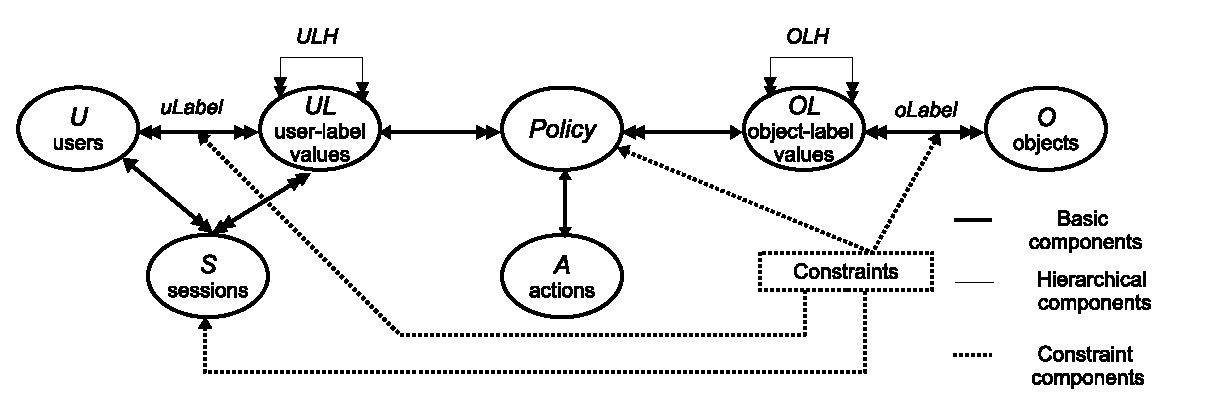
\includegraphics[width=.9\textwidth]{labac-1-11}
		\caption{Components of LaBAC}
		\label{fig:labac}
	\end{figure*}
	

	\begin{figure}
		\centering
		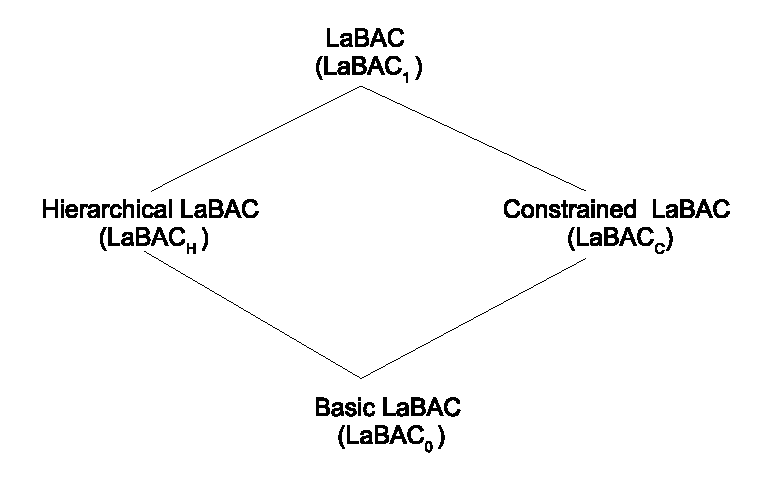
\includegraphics[width=.5\textwidth]{labac-family}
		\caption{Family of LaBAC models}
		\label{fig:labac-family}
	\end{figure}
		

%\section{\eapABAC{} Family}
\section{Single Attribute Enumerated Authorization-Policy Models}

	\label{sec:model}


Here we describe the \eapABAC{} family of models  along with formal definitions. \eapABAC{} uses one user-attribute named $\uLabel$ and one object-attribute named $\oLabel$. We define these attributes with predefined semantics. While attributes in general have open-ended semantics, labels ($\uLabel$ and $\oLabel$) are associated with specific semantics. For example, in general, attributes can be set-valued (e.g. roles or clearance) or atomic valued (e.g. age). An attribute value (eg. role, clearance) can be assigned by administrators, self-asserted (e.g. date of birth), or derived from other attributes (e.g. age can be derived from date of birth). Moreover, value of attributes can be ordered or unordered.  On the other hand, labels are set-valued, values are partially ordered and are assigned by administrators. 



We specify \eapABAC{} as a family of models. The basic EAP model (\clabac) presents the minimum elements to define an EAP model. Additionally, we add hierarchies and constraints in \hlabac{} and  \consLabac{} respectively.  \labacOneOneOne{} combines both the hierarchical and constrained models. The components of the \eapABAC{} models are shown in Figure \ref{fig:labac} and the family of the models is schematically presented in Figure \ref{fig:labac-family}.
	% Please add the following required packages to your document preamble:
% \usepackage{booktabs}
\begin{table}
	\centering
	\caption{ \clabac{} Model} %\vspace*{3pt}
	\label{tab:labac-definition}
		\begin{tabular}{|l|}						
		\hline					
				\multicolumn{1}{|c|}{\underline{\textit{I. Sets and relations }}}\\			
				- $U, O$ and $S$ (set of users, objects and sessions resp.)  \\
				- $UL$, $OL$ and $A$ (finite set of user-label values, \\ \hfill object-label values and action resp.) \\
				- $uLabel$ and $oLabel$ (label functions on users and \\ \hfill objects).  $\uLabel: U \to 2^{\UL}$;   $\oLabel: O \to 2^{\OL}$ \\			
				- $\creator: S \to U$, many-to-one mapping from $S$  to $U$ \\
				- $\sessionLabels: S \to 2^{UL}$, mapping from $S$   to    $uLabel$  values. \\ \hfill
				$\sessionLabels(s) \subseteq   uLabel(\creator(s)) $ 	\\ 
				$\langle$ see Section \ref{sec:session-management} for session management functions $\rangle$\\
			%	\hfil [session management functions] \\ 
				\\ \multicolumn{1}{|c|}{\underline{\textit{II. Policy components}}} \\	
				-  $\Policy_a \subseteq \ULV \times  \OLV$,  for action $a \in A$. \\
				- $\Policy = \{ \Policy_a | a \in A  \}$ \\ \\			
				
				\multicolumn{1}{|c|}{\underline{\textit{III. Authorization function}}} \\						
				- \request(s:S,\amem:A,\objmem:O) =	 
					$\exists ul \in \sessionLabels(s) ,$ \\ \hfill $ \exists ol \in oLabel(o)$  $[ (ul,ol) \in$ $\textit{\policy}_a ]  $  		
			
 \\ \hline	
	\end{tabular}
	
\end{table}

%mod


	
\subsection{Basic \eapABAC{} Model}
The elements represented by solid bold lines in Figure \ref{fig:labac} represent the Basic \eapABAC{} Model (\clabac{}). In this model, a set of users, objects and actions (finite set) are represented by $U, O$ and $A$ respectively. Users are associated with a label function named $\uLabel$ and objects are associated with another label function, $\oLabel$. The function $\uLabel$ maps a user to one or more values from the finite set  $UL$ (represented by the double headed arrow from users to UL) and similarly $\oLabel$ maps one object to one or more values from the finite set $OL$ (represented by the double headed arrow from objects to OL). The double headed arrow from $UL$  to users and $OL$ to objects indicate that one user-label value can be associated with more than one user and one object-label value can be associated with more than one object. 

		
 	\begin{figure}
 		\centering
 		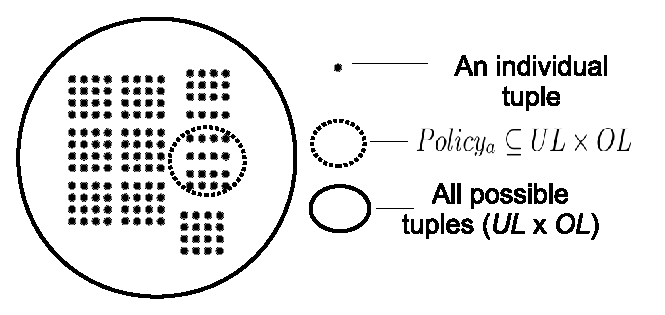
\includegraphics[width=.6\textwidth]{ABAC16/tuples-vs-policy}
 		\caption{Authorization policy as subset of tuples}
 		\label{fig:policy-vs-tuples}
 	\end{figure}	


	
Sessions are denoted by the set $S$. There is a one-to-many mapping from users to sessions. While a user  may have many $\uLabel$ values assigned to him, he can choose to activate any subset of the assigned values in a session. The relation (and function) $\creator$ and $\sessionLabels$ maintain mapping from sessions to users and sessions to $\uLabel$ values respectively.  The $\creator$ and $\sessionLabels$ functions are formally defined in Segment I of Table \ref{tab:labac-definition}. 



In \eapABAC{}, for each action, $a \in A$ we define only one policy, denoted $Policy_a$. A policy is comprised of a subset of tuples from the set of all tuples $UL\times OL$. Relationship between a policy and tuples is schematically shown  in Figure \ref{fig:policy-vs-tuples}. In defining policies, a policy may contain many tuples and a tuple $(ul,ol) \in UL\times OL$ can be used in more than one policy. Thus, a many-to-many relation exists between policies and tuples. Finally, the set \textit{\Policy} contains all individual policies for each action $a \in A$. The formal definition of \textit{\Policy{}} is shown in Segment II of Table \ref{tab:labac-definition}.

The authorization function $\request(s, a, o)$ allows  an access request by a  subject $s \in S$ to perform an action $a \in A$ on an object $o \in O$ if all the following conditions are satisfied - $s$ is assigned a value $ul$;  $o$ is assigned a value $ol$ and the policy for action $a$ contains the tuple $(ul,ol)$. The formal definition of the authorization function is given in Segment III of Table \ref{tab:labac-definition}.


	
		
 	\begin{figure}
 		\centering
 		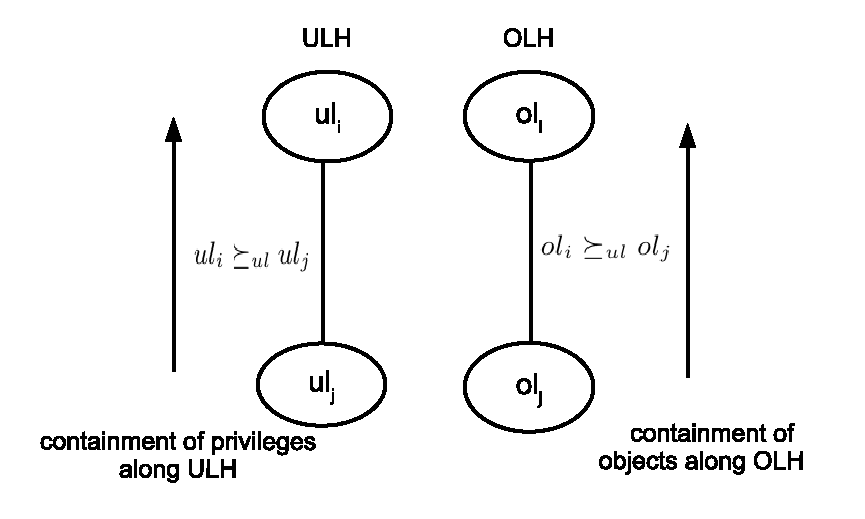
\includegraphics[width=.7\textwidth]{ABAC16/direction-of-implication}
 		\caption{ULH and OLH}
 		\label{fig:direction-of-implication}
 	\end{figure}

		
	
	
	\subsection{Hierarchical \eapABAC{}}
	Hierarchical \eapABAC{} model (\hlabac ) introduces user-label hierarchy ($ULH$) and object-label hierarchy ($OLH$) in addition to the components of \clabac{}. Some elements in \clabac{} are modified in \hlabac{}. The additions and modifications in \hlabac{} from \clabac{} are shown in Table \ref{tab:labach-definition}.
	
	Hierarchy is a convenient way of ranking users and objects. \eapABAC{} achieves ranking on users through $ULH$ and ranking on objects through $OLH$. For two user-label values, $ul_i$ and $ul_j$, when we say $ul_i$ is senior to $ul_j$ (written as $ul_i \udominate ul_j$), we mean that users assigned to $\uLabel$ value $ul_i$  can also exercise all privileges of users who are assigned to value $ul_j$. Similarly, for two object-label values, $ol_i$ and $ol_j$, when we say $ol_i$ is senior to $ol_j$ (written as $ol_i \odominate ol_j$), we mean that objects assigned to value $ol_j$ are also considered as inherited objects for value $ol_i$ for the purpose of authorization. The direction for the containment of privileges and objects along the hierarchy of $ULH$ and $OLH$ is shown in Figure \ref{fig:direction-of-implication}. For containment of objects, in Figure \ref{fig:implied-policy} objects that are assigned value `public', are also considered to be objects that are assigned  value `protected'.
	
	% For example, in Figure \ref{fig:implied-policy}, $protected \odominate public$ and   $ULH$ and $OLH$ is explained in Figure \ref{fig:direction-of-implication}.
	
	When we assign a tuple $(ul_m,ol_n)$ in a policy $\Policy_a$, additional tuples are also implied for $\Policy_a$ because of user-label and object-label value hierarchy. We identify these implied tuples with the notion of a new set $\impliedPolicy$. The implied policy  $\impliedPolicy_a$ includes all tuples of $\Policy_a$ and extra tuples that are implied by every tuples of $\Policy_a$. 
	
	%There is a one-to-one mapping between policies and implied policies.
	

	
		
		% Please add the following required packages to your document preamble:
% \usepackage{booktabs}
\begin{table}
	\centering
	 \captionsetup{justification=centering}
	 \caption{\hlabac{} Model (additions and modifications to \clabac{})}
	%\caption{  } %\vspace*{3pt}
	\label{tab:labach-definition}
		\begin{tabular}{|l|}						
		\hline								
			\multicolumn{1}{|c|}{\underline{\textit{I. Sets and relations}}} \\		
			%\multicolumn{1}{|c|}{\underline{\textit{(in addition to the basic model)}}} \\		
				  - $\ULH \subseteq \ULV \times \ULV$, partial order ($\succeq_{ul}$) on $UL$  \\
					
	              - $\OLH \subseteq \OLV \times \OLV$, partial order ($\succeq_{ol}$) on $OL$  \\ 
				  - $\sessionLabels(s) \subseteq   \{ ul' | ul \in uLabel(\creator(s)) \land ul \udominate ul' \}$		\\   \\						  				 			 	
		
			\multicolumn{1}{|c|}{\underline{\textit{II. Implied policy}}} \\
				- $\impliedPolicy_a = \{ (\ulvmem_i, \olvmem_j) |  \exists (\ulvmem_m, \olvmem_n) \in \policy_a$[  $ \ulvmem_i \udominate \ulvmem_m \land \olvmem_n \odominate \olvmem_j] \}$	\\ \hfil (explained in Figure \ref{fig:implied-policy})	\\ \\
				
				%- $\textit{\effectivePolicy}_a$ $ = \policy_a \cup \impliedPolicy_a$ \\\\
					
		 	\multicolumn{1}{|c|}{\underline{\textit{III. Authorization function}}} \\
				 
				 	- \request(s:S,\amem:A,\objmem:O) $\equiv$	 
				 	$\exists ul \in \sessionLabels(s) ,$  $ol \in oLabel(o)$  $[ (ul,ol) \in$ $\textit{\impliedPolicy}_a ]  $ \\					 
 \hline	
	\end{tabular}
	
\end{table}

%mod



	
 	\begin{figure}[h]
 		\centering
 		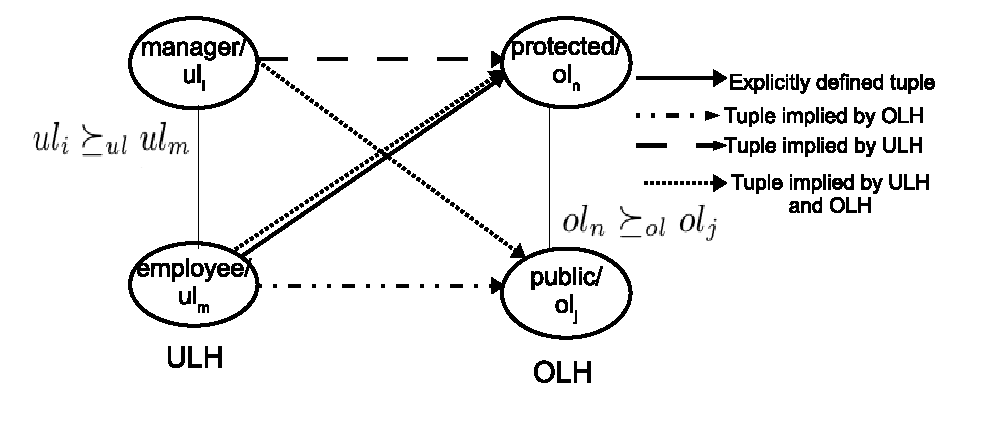
\includegraphics[width=1\textwidth]{ABAC16/implied-policy}
 		\caption{Policy and implied policy}
 		\label{fig:implied-policy}
 	\end{figure}
	
	Implied policy is  explained in Figure \ref{fig:implied-policy}.  For a policy, $\Policy_a = \{(employee, protected)\}$, corresponding implied policy is $\impliedPolicy_a=\{(manager, protected),$ \\$ (manager, public), (employee, protected), (employee, public)\}$. Figure \ref{fig:implied-policy}, further classifies tuples into tuples implied by $ULH$, or $OLH$ or both. Note that authorization function and session function are also modified in Table \ref{tab:labach-definition} to accommodate $ULH$ and $OLH$.
	


	
	
	
	%
 	\begin{figure} 
 		\centering
 		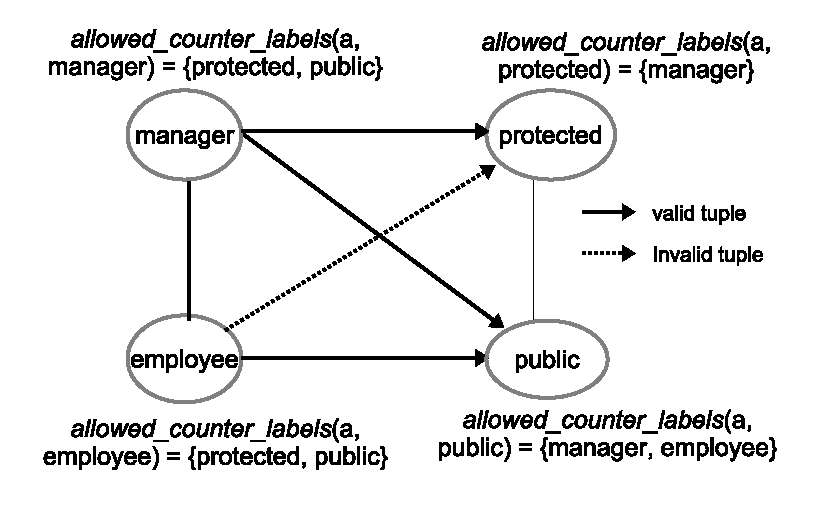
\includegraphics[width=.4\textwidth]{bound-function-explained}
 		\caption{Policy constraints explained with constraint function - \allowedLabels()}
 		\label{fig:bound-function-explained}
 	\end{figure}
	
	\subsection{Constrained \eapABAC{}}
	A general treatment of assignment constraints in ABAC has been covered in  \cite{abcl}. Similarly, role based authorization constraints have been extensively studied in \cite{rcl}.	
	In this section, we specify constraints for the \eapABAC{} model. 
	
	We scope constraints as  means of restricting administrative or user actions. We define two types of constraints - assignment constraints and  policy constraints. Assignment constraints put constraints on user to user-label value assignments,  object to object-label value assignments and session-label value assignments. An example of user-label value assignment constraint is that a user cannot be assigned all of the following values $\{manager, director,$  $employee\}$.  An example of object-label value assignment constraint is that an object cannot be assigned both values - \textit{protected} and \textit{public}. An example of session-label value assignment constraint is that both \textit{manager} and \textit{director} values cannot be activated in the same session.	 Policy constraints, on the other hand,  prevent certain tuples in policies. For example, policy constraints may enforce that an \textit{employee} can never access \textit{protected} objects by restricting the tuple \textit{(employee, protected)}.  
	
	
	\begin{table}
	\centering
	\captionsetup{justification=centering}
	\caption{\consLabac{} Model \newline (Additions and modifications to \clabac{})} %\vspace*{3pt}
	\label{tab:constraint-definition}
%	\begin{tabular}{|l|l|}
%		\hline
		\begin{tabular}{|l|}						
			\hline					
				
				  \multicolumn{1}{|c|}{\underline{\textit{I. Components added from \clabac{}}}} \\								 
					\textit{uLabel value assignment constraint:}\\
						  - CUL = a collection of conflicting user-label values, \\ \hfil $\{ CUL_1, CUL_2, ... CUL_n \}$    where $CUL_i = \{ ul_1, ... ul_k\}$ \\		
 					\textit{oLabel value assignment constraint:}\\
						    - COL = a collection of conflicting object-label values,\\ \hfil $\{ COL_1, COL_2, ... COL_n \}$    where $COL_i = \{ ol_1, ... ol_k\}$ \\
				    \textit{Session value assignment constraint:}\\
					    	 - CSL = a collection of conflicting user-label values, \\ \hfil $\{ CSL_1, CSL_2, ... CSL_n \}$    where $CSL_i = \{ ul_1, ... ul_k\}$ 	\\ 
								  
					\textit{Policy constraint:}\\
						 % - $\allowedLabels(a:A, l:UL/OL) \to 2^{UL/OL}$,  \\ \hfill allowed oLabel values for   given uLabel values \\ \hfill  and vice-versa for action $a$.	\\
						 - $\restrictedTuples \subseteq UL \times OL$ \\
						  
			\\ \multicolumn{1}{|c|}{\underline{\textit{II. Derived components}}}	  \\
						  %- $\textit{\policyBound}_a =$ \\ \hfill $ \{ (ul,ol) | \exists ul \in UL \land ol \in \allowedLabels(a,ul)\}  \cap$  \\ \hfill  $\{ (ul,ol) | \exists ol \in OL \land ul \in \allowedLabels(a,ol)\}$  \\    \\				
						  - $\policyBound = (UL \times OL) \setminus \restrictedTuples$ \\
			 
			
			\\ \multicolumn{1}{|c|}{\underline{\textit{III. Authorization function}}} \\						
					- \request(s:S,\amem:A,\objmem:O) =	 
					$\exists ul \in \sessionLabels(s) ,$ \\ \hfill $ \exists ol \in oLabel(o)$  $[ (ul,ol) \in$ $\textit{\policy}_a \cap \policyBound_a  ]  $  					  
			 
				 	
			 %	\multicolumn{1}{|c|}{\underline{\textit{VI. Sample Enforcement of Assignment Constraints}}} \\
			%		- $ | labels(s) \cap OneElement(CSL) | = 1$, only one  user-label \\ \hfill value can be activated in a session. 
 \\ \hline	
	\end{tabular}
	
\end{table}
	% Please add the following required packages to your document preamble:
% \usepackage{booktabs}
\begin{table}
	\centering
	\caption{ \combinedEAP{} model} %\vspace*{3pt}
	\label{tab:labac-complete-definition}
		\begin{tabular}{|l|}						
		\hline					
				\multicolumn{1}{|c|}{\underline{\textit{I. Basic Components }}}\\	\\		
				- $U, O$ and $S$ (set of users, objects and sessions resp.)  \\
				- $UL$, $OL$ and $A$ (finite set of user-label values, object-label values and action resp.) \\
				- $uLabel$ and $oLabel$ (label functions on users and  objects). \\ \hfil  $\uLabel: U \to 2^{\UL}$;   $\oLabel: O \to 2^{\OL}$ \\				
				- $\ULH \subseteq \ULV \times \ULV$, partial order ($\succeq_{ul})$ on $UL$  \\	
				- $\OLH \subseteq \OLV \times \OLV$, partial order ($\succeq_{ol}$) on $OL$  \\ 
				- $\creator: S \to U$, mapping from $S$  to $U$ \\
				- $\sessionLabels: S \to 2^{UL}$, mapping from $S$   to $uLabel$  values.\\ \hfill	$\sessionLabels(s) \subseteq   \{ ul' | ul \in uLabel(\creator(s)) \land ul \udominate ul' \}$			\\    			  
			    %- $\allowedLabels(a:A, l:UL/OL) \to 2^{UL/OL}$,  \\ \hfill allowed oLabel values for   given uLabel values \\ \hfill  and vice-versa for action $a$.	\\\\
 			   - $\restrictedTuples \subseteq UL \times OL$ \\
 			   - \textit{CUL, COL, CSL} (conflicting set of $\uLabel, \oLabel$ and session-label values) \\
 			   $\langle$ see Section \ref{sec:session-management} for session management functions $\rangle$\\
			    
			   \\	\multicolumn{1}{|c|}{\underline{\textit{II. Policy components}}} \\	\\
			   	-  $\Policy_a \subseteq \ULV \times  \OLV$,  for action $a \in A$. \\
			   	- $\Policy = \{ \Policy_a | a \in A  \}$ \\ \\
			    
			    \multicolumn{1}{|c|}{\underline{\textit{III. Derived components}}} \\\\
			    - $\impliedPolicy_a = \{ (\ulvmem_i, \olvmem_j) |  \exists (\ulvmem_m, \olvmem_n) \in \policy_a$[ $ \ulvmem_i \udominate \ulvmem_m \land \olvmem_n \odominate \olvmem_j] \}$	\\
			     - $\textit{\policyBound} = (UL \times OL) \setminus \restrictedTuples$ \\
			    
			    
				\\ \multicolumn{1}{|c|}{\underline{\textit{IV. Authorization function}}} \\ 	\\					
				- \request(s:S,\amem:A,\objmem:O) $\equiv$	 
					$\exists ul \in \sessionLabels(s), $ $\exists ol $ \\ \hfill   $ \in oLabel(o) [ (ul,ol) \in$ $\textit{\impliedPolicy}_a \cap  \textit{\policyBound}]  $  		
			
 \\ \hline	
	\end{tabular}
	
\end{table}

%mod


		
		 
		 
	Assignment constraints are specified by defining a set of conflicting $\uLabel$, $\oLabel$ and \textit{session} values denoted by $COL$, $CUL$ and $CSL$ respectively in Table \ref{tab:constraint-definition}.  The constraint that an object cannot be assigned both values - `protected' and `public' is specified as $COL=\{\{public, protected\}\}$ and $ |\oLabel(o) \cap OneElement(COL)| \le 1$ where function $OneElement()$ returns one element from its input set. (we use the same concept of \textit{OneElement()} from \cite{rcl}).  Similarly, other  assignment constraints can also be formulated. Note that user-label value assignment constraints can be used to configure  Static Separation of Duty, while session constraints can be used to enforce some aspects of  Dynamic Separation of Duty \cite{dsod}.


 	\begin{figure}
 		\centering
 		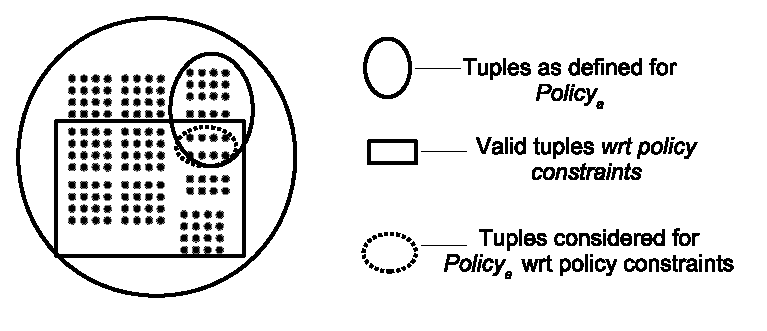
\includegraphics[width=.6\textwidth]{ABAC16/tuples-vs-valid-tuples}
 		\caption{Restricting policies with policy constraints}
 		\label{fig:tuples-vs-valid-tuples}
 	\end{figure}	


	Policy constraints are defined by using \textit{\restrictedTuples}.  For a tuple, $(ul_r,ol_r) \in \restrictedTuples$, if it is included in a policy, $\Policy_a$, it would be ignored in the computation of authorization decision. For convenience we define a derived set \textit{\policyBound} as all possible tuples minus \textit{\restrictedTuples}. \textit{\restrictedTuples} and \textit{\policyBound} are defined in Table \ref{tab:constraint-definition}. Policy constraint is explained schematically in Figure \ref{fig:tuples-vs-valid-tuples}.
	
	In \consLabac{}, we include constraint policies beyond authorization policies. While, authorization policies establish relationship only between user-label and object-label values (along with actions), constraint policies go beyond. For example, constraint policies may consider relationship between \textit{UL} and \textit{OL} (policy constraints), $UL$ and $UL$ (\textit{\uLabel/session} value assignment constraints), $OL$ and $OL$ (\textit{\oLabel} value assignment constraints), \textit{S} and \textit{UL} (cardinality constraints on session value assignments) and so on.  As a result, constraint policies in \consLabac{} include logical formulas as well as enumerated tuples.
	
	
	
	
	\subsection{The Combined Model (\labacOneOneOne{})}
	
	The combined model, \labacOneOneOne{} (shown in Table \ref{tab:labac-complete-definition}), combines elements from both \hlabac{} and \consLabac{} models.  Segment I of Table \ref{tab:labac-complete-definition} presents all basic sets and relations. Policy components and derived components are shown in Segment II and  III respectively. Finally, authorization decision function is defined in Segment IV.
	


\section{Functional Specification of \eapABAC{} models}
		


%\subsection{Functional Specification}
\label{sec:session-management}
\input{ABAC16/session-functions.tex}



\eapABAC{} allows users to create or destroy sessions, and assign/remove values from an existing session. Table \ref{tab:session-management} presents user-level \textit{\sessionLabels{}} functions for managing sessions in \clabac{}. Each function is presented with formal parameters (given in the first column), necessary preconditions (in the second column) and resulting updates (in the third column).  The function $\createSession()$ creates a new session with given values, $\deleteSession()$ deletes an existing session, $\assignValues()$ assigns values in an existing session, and $\removeValues()$ removes values from an existing session. 

%First column in the table shows function names along with formal parameters, second column defines precondition which must be satisfied for the function to be executed. The third column describes updates in the LaBAC sets and relations once corresponding function is executed.

In \hlabac{}, we modify condition of the session functions from Table \ref{tab:session-management} to accommodate  that in a session created by a user, he can choose from the values he is assigned to or junior values. The modified conditions are given in Table \ref{tab:session-in-hlabac}. We specify an additional condition with each session function  in \consLabac{} and \labacOneOneOne{}.  For example, with $\createSession()$,  we specify a boolean function $f_{\createSession}()$ as additional precondition which must also be true. The definition of these boolean functions are  open-ended to be able to configure any session constraints. The difference between session functions in \consLabac{} and \labacOneOneOne{} is that the former does not consider hierarchy on user-label values whereas the later does. Table \ref{tab:session-in-consLabac} and \ref{tab:session-in-labacOne} show session functions in \consLabac{} and \labacOneOneOne{} respectively. Table \ref{tab:example-f-create-session} presents some examples of constraints specified with $f_{\createSession}()$ function.  \textit{Example 1} uses an enumerated policy, $\Policy_{\createSession}$. It specifies that in order to create a session and assign values to the session, a user must be assigned to value $\createReq$. \textit{Example 2} enforces the constraint that no more than one conflicting $\uLabel$ values can be activated in a session. \textit{Example 3} imposes that a user cannot have more than some bounded number of sessions.

Note that creation and deletion of objects, updating object-label values by sessions are outside the scope of \eapABAC{} operational models presented here. One reason behind is that, \eapABAC{} only focuses on attributes. It can be extended to include object creation and modification along the line of $ABAC_{\alpha}$ \cite{abacAlpha}. See Table \ref{tab:lbac-in-labac} for example.

\input{ABAC16/session-in-hlabac.tex}

\input{ABAC16/session-in-clabac.tex}

\input{ABAC16/additional-session-constraints.tex}



\input{ABAC16/example-f-create-session.tex}



	 \input{policy-table-enumeration.tex}
\subsection{Quantifying \labacOneOneOne{} authorization policies}
In \eapABAC{}, we define one authorization policy per action.  A policy can take any subset of all possible tuples. Thus, different number of ways to define a policy  is the size of the power set of all possible tuple as shown in Figure \ref{fig:policy-vs-tuples}.  Table \ref{tab:policy-enumeration} shows possible number of enumerated authorization policies in \labac{}.





\section{Configuring Traditional Models in  \eapABAC{}}
	\label{sec:configuration}
	In this section, we establish relationship between \eapABAC{} and traditional access control models. We first show that \eapABAC{} is equivalent to \twoSortedRBAC{} which is an enumerated policy model for RBAC. Additionally, we show how to configure RBAC and LBAC using \eapABAC{} model.
\subsection{Equivalence of \eapABAC{}  and \twoSortedRBAC{} }
	%\section{Equivalence of LaBAC and \newline 2-sorted-RBAC}
\label{sec:equivalence}
\twoSortedRBAC{} \cite{two-sorted-rbac} is an interesting extension of Role Based Access Control which breaks the duality of roles (users and permissions perspectives) into proper roles ($\properRole$) as group of users and demarcation ($\demarcation$) as group of permissions. User inheritance is maintained with proper role hierarchy ($\properRoleHierarchy$) and permission inheritance is maintained with demarcation hierarchy ($\demarcationHierarchy$). The connection between proper roles and demarcation is maintained by the grant relation ($G$) which enumerates (proper role, demarcation) pairs. For example, for proper roles and demarcations given in Figure \ref{fig:two-sorted-rbac-example}, G includes following tuples - \{(manager, red), (employee, amber)\}. Note that \twoSortedRBAC{} \cite{two-sorted-rbac} also includes negative roles and demarcations which we do not consider here.



\twoSortedRBAC{} is compelling in many ways. It introduces a higher administrative level (through grant relation) for access management. User-role assignment ($UR^+ \subseteq U \times \properRole$) and demarcation-permission assignment ($PD^+ \subseteq P \times \demarcation$), along with administration of grant relation can be carried out more independently and distributively. Moreover, the authors shows that, \twoSortedRBAC{} enables many-to-many administrative mutations which leads to organizational scalability.  In many-to-many mutation, by granting a (proper role, demarcation) pair, all users in the proper role get all  permissions in the demarcation which, as the authors shows cannot be achieved by standard RBAC \cite{nist-rbac}.


  \begin{figure}
 	\centering
 	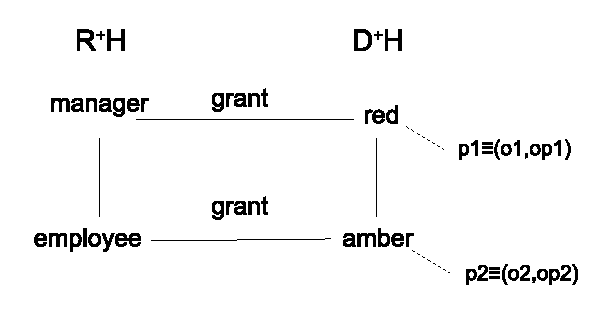
\includegraphics[width=.7\textwidth]{ABAC16/two-sorted-rbac-example}
 	\caption{An example of Two-sorted-RBAC}
 	\label{fig:two-sorted-rbac-example}
 \end{figure} 

 

The benefits of \twoSortedRBAC{} can also be realized through LaBAC. For example, user to $\uLabel{}$ value assignments, object to \oLabel{} value assignments and authorization policies are analogous to $\properRoleHierarchy$, $\demarcationHierarchy$ and grant relation in \twoSortedRBAC{} and  can also be carried out independently. On the other hand, many-to-many administrative mutation can also be achieved. For example, the LaBAC policy, $\Policy_{op1}\equiv \{(manager, (red,op1))\}$ in Figure \ref{fig:two-sorted-rbac-to-labac-example},  enables every   $manager$ to perform operation $op1$ on every object labeled with  $(red,op1)$. 

 \begin{figure}
 	\centering
 	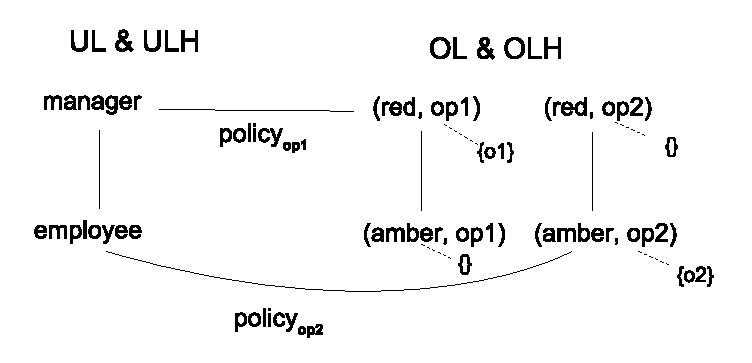
\includegraphics[width=.7\textwidth]{ABAC16/two-sorted-rbac-to-labac-example}
 	\caption{An example of Two-sorted-RBAC configured in LaBAC}
 	\label{fig:two-sorted-rbac-to-labac-example}
 \end{figure}
 


 \begin{table}
	\centering
	\caption{ \twoSortedRBAC{} in \hlabac} %\vspace*{3pt}
	\label{tab:two-sorted-rbac-in-labac-table}
	\begin{tabular}{|l|}						
		\hline					
		\multicolumn{1}{|c|}{\underline{\textit{I. \twoSortedRBAC{} components }}}\\	\\			 
		 -  $S, OBS, OPS$, $\roles, \RH$, $\demarcation, \DeH$,   (users, objects,   operations, proper roles, \\ \hfill role hierarchy, demarcation  and demarcation hierarchy respectively). \\
		 -  $PRMS = {(OBS \times OPS)}$, the set of permissions  \\		 
		 -  $\SR \subseteq S \times \roles$  \\
		 -  $\PD \subseteq PRMS \times \demarcation$ \\	 
		 - $G \subseteq \roles \times \demarcation$\\
		\\ \multicolumn{1}{|c|}{\underline{\textit{II. Construction in \hlabac{}}}} \\ \\
		 	-  $U = S, O = OBS, A = OPS $ \\ 
		 	- $UL=\roles, ULH=\RH$\\		  
		 	- $ OL = \demarcation \times OPS$\\
		 	- $OLH= \{ ((d_i, op_i), (d_j, op_j)) | d_i  \succeq d_j \land op_i = op_j\}$\\
		 	-  $\uLabel(u) = \{ r | (s,r) \in \SR \}$ \\		 	
		 	-  $ \oLabel(o) = \{ (d,op) | ((o,op),d) \in PD \}$\\		 	 	
		 	-  $\policy_{op_i} = \{ (r_i, (d_j,op_j) ) |  (r_i,d_i) \in G \land$ $((o,op_i),d_i)  \in \PD \} $ \\
		 \hline	
	\end{tabular}	

	
\end{table}

 
 In fact, LaBAC is similar to \twoSortedRBAC{} in spirit. While \twoSortedRBAC{} is more role oriented, LaBAC is attribute oriented. In the following of this section, we show equivalence of LaBAC and \twoSortedRBAC{} with respect to their theoretical  expressive power. In order to establish the equivalence, we show that any instance of \twoSortedRBAC{} can be expressed in LaBAC and vice-versa.

 
 
Figure  \ref{fig:two-sorted-rbac-to-labac-example} is an example showing configuration of a \twoSortedRBAC{} instance (given in Figure \ref{fig:two-sorted-rbac-example}) in LaBAC. In Figure  \ref{fig:two-sorted-rbac-to-labac-example}, user-label values and its hierarchy directly corresponds to roles and role hierarchy in Figure \ref{fig:two-sorted-rbac-example}. On the other hand, object-label values correspond to Cartesian product of $\demarcation$ and $OPS$.   An object-label value $(d_i, op)$ dominates another object-label value $(d_j, op)$, if demarcation $d_i$ dominates demarcation $d_j$. For example, for demarcations \{$red$, $amber$\} and operations $\{op1,op2\}$ (of Figure \ref{fig:two-sorted-rbac-example}), four object-label values have been defined where $(red,op1)$ dominates $(amber,op1)$ because $red$ dominates $amber$.  For an object-label value $(d,op)$, we assign $(d,op)$ to the object $o$ to if $(o,op)$ is a permission in demarcation $d$. For example, object $o1$ is assigned the value $(red,op1)$ because $(o1,op1)$ is  a permission in demarcation $red$.  On the other hand, user-label values assigned to a user corresponds to his assigned proper roles. Finally, having assigned object-label and user-label values, for each grant relation $(r,d) \in G$,  we specify authorization policy $Policy_{op} \equiv \{(r,(d,op))\}$ so that object labeled with $(d,op)$ are accessed by users with role $r$ for operation $op$. For example, for the grant relation $(manager,red)$ in Figure \ref{fig:two-sorted-rbac-example}, we create a policy $Policy_{op1} \equiv \{(manager, (red,op1))\}$. We do not create  policy $Policy_{op2} \equiv \{(manager, (red,op2))\}$ because there is no permission defined with operation $op2$ in demarcation $red$. Table \ref{tab:two-sorted-rbac-in-labac-table} formally  shows this configuration.
 

 
 %  \begin{figure}[!htbp]
 	\centering
 	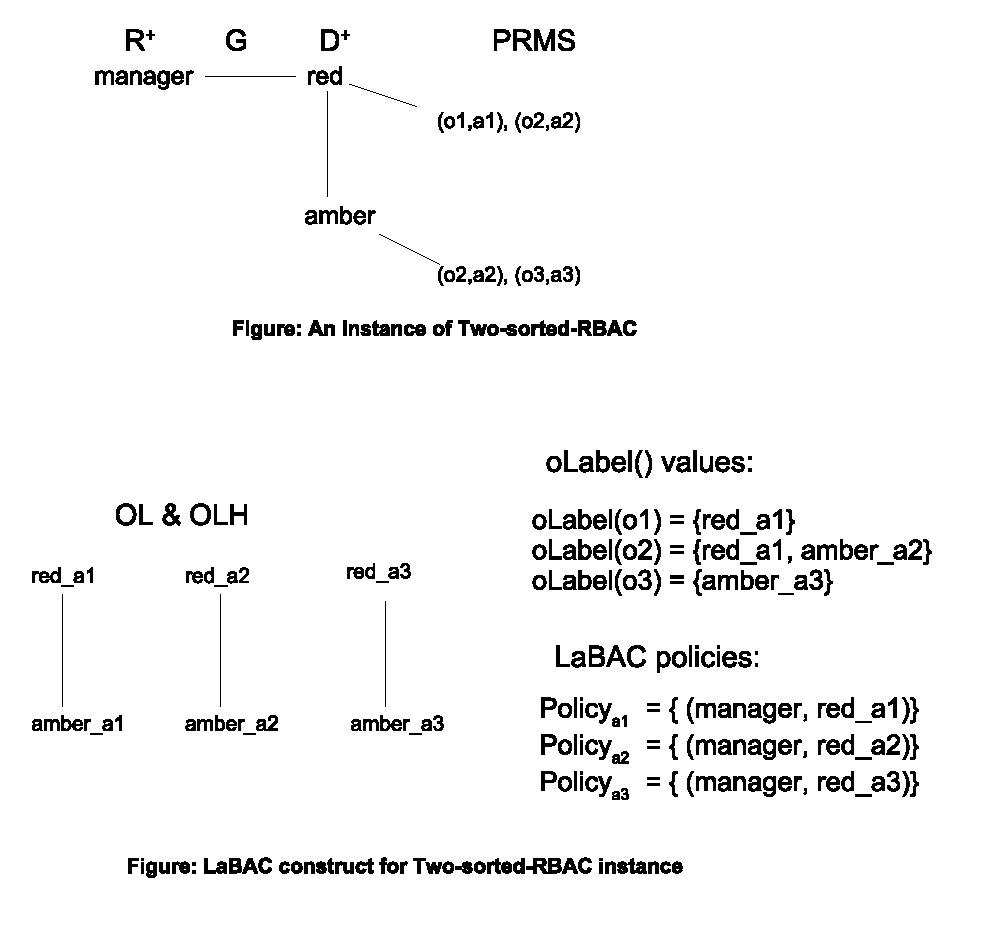
\includegraphics[width=.6\textwidth]{two-sorted-labac-example-diagram}
 	\caption{A $RBAC_1$ instance of role and perms.}
 	\label{fig:two-sorted-labac-example-diagram}
 \end{figure}
 
 \begin{table}
	\centering
	\caption{ \hlabac{} in \twoSortedRBAC{} } %\vspace*{3pt}
	\label{tab:labac-in-two-sorted-rbac-table}
	\begin{tabular}{|l|}						
		\hline					
			\multicolumn{1}{|c|}{\underline{\textit{I. \hlabac{} components}}} \\
			-  $U, O,  A$ (set of users, objects and actions resp.) \\ 
%			- $UL, OL, ULH,  OLH$ (uLabel and oLabel values, \\ \hfill uLabel and oLabel value hierarchy  resp.) \\		  
%			-  $\uLabel()$, user to user-label value assignment relation \\		 	
%			-  $\oLabel()$, object to object-label value assignment relation \\
%			-  $\policy_{a}$, LaBAC authorization policies for $a \in A$\\\\
			- $UL, OL, ULH,  OLH$ (uLabel values, oLabel values, \\ \hfill uLabel and oLabel value hierarchy  resp.) \\		  
			-  $\uLabel: U \to 2^{UL}$, $\oLabel: O \to 2^{OL}$ \\
			-  $\Policy_{a}$, authorization policy for action $a \in A$\\
		
		\\ \multicolumn{1}{|c|}{\underline{\textit{II. Construction in \twoSortedRBAC}}}\\	
		- $S=U, OBS=O, OPS=A$\\			 
		 - $\properRole = UL$, $\properRoleHierarchy = ULH$ \\ 
 		 - $\demarcation = OL$, $\demarcationHierarchy = \{\}$ \\ 
 		 - $\SR = \{ (u,r) | r \in uLabel(u)\}$\\
 		 - $\PD = \{ ((o_i, a_i), ol) | \exists (ul,ol) \in \policy_{a_i} \land$ \\ \hfill $ol' \in oLabel(o_i) \land ol \odominate ol'\}$ \\
 		 - $G = \{ (ul,ol) | (ul,ol) \in \policy_a  \}$\\
		\hline	
	\end{tabular}	

	
\end{table}

 
 
 
 Configuration of \hlabac{} in \twoSortedRBAC{} is given in Table \ref{tab:labac-in-two-sorted-rbac-table}. Segment I represents elements of LaBAC model and Segment II shows the configuration.  In the configuration, user-label values and its hierarchy are used as proper roles and proper role hierarchy. Object-label values are used as names for demarcations. For an object-label value $ol\in OL$, let $O_{ol}$ be the objects labeled with $ol$. For each policy $policy_{op} \equiv \{(ul, ol)\}$ in LaBAC, we create a grant relation $(ul,ol)$ in \twoSortedRBAC{}. Further, assign permission (o,op) in demarcation named $ol$ for $o \in O_{op}$. Note that \twoSortedRBAC{} does not distinguish between users and sessions as we do in LaBAC. For this reason, we omit LaBAC sessions while showing equivalence with \twoSortedRBAC{}.
 
 
 

  
  Here we use \hlabac{} to configure \twoSortedRBAC{} for convenience. In fact,  \clabac{} is the minimalistic model that is equivalent to \twoSortedRBAC{}. In Figure \ref{fig:expressiveness-spectrum}, we show summary of expressive power of different LaBAC models. The dashed box represents the minimalistic LaBAC model required to configure other models and solid box represents the LaBAC model that we use for our convenience. 

%We acknowledge the more formal  approach of \textit{state matching reduction} or simply \textit{reduction} \cite{tripli} for establishing equivalence between access control models. For simplicity and absence of state transition functions (administrative models) for some models discussed here, we adopt a simplified and conventional approach for the establishment of  equivalence.

The construction of Tables \ref{tab:two-sorted-rbac-in-labac-table} and \ref{tab:labac-in-two-sorted-rbac-table} and other constructions given in the rest of this paper can be cast in the formal approach of \cite{tripli}. So, these models are equivalent in the sense of state-matching reduction. 

   \begin{figure}
 	\centering
 	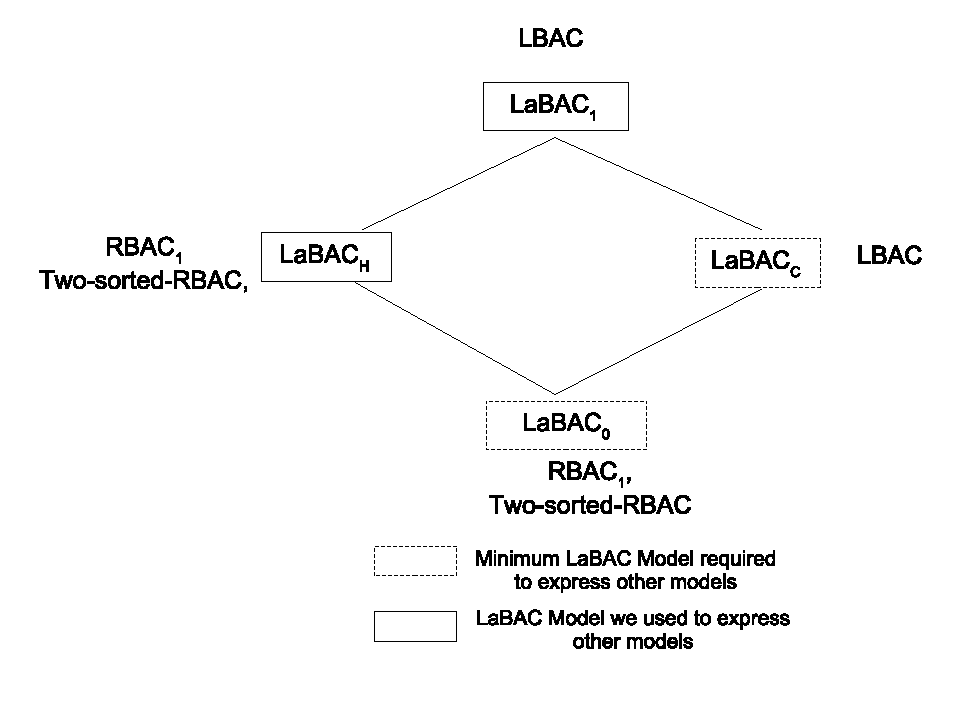
\includegraphics[width=.8\textwidth]{ABAC16/expressiveness-spectrum}
 	\caption{Expressiveness of LaBAC models}
 	\label{fig:expressiveness-spectrum}
 \end{figure}
 

\subsection{Configuring LBAC in \eapABAC{}}
	%

%\section{LBAC and RBAC in  LaBAC}
\label{sec:configuration}
In this section, we configure LBAC \cite{lbac} and RBAC \cite{rbac}  using \labacOneOneOne{}. For each configuration, we additionally show the required number of label values and authorization policies. 

\input{ABAC16/lbac-in-labac.tex}
 %\input{rbac-labac-configuration-explained.tex}
 \input{rbac-in-labac.tex}



%\input{dac-in-labac.tex}


In this section, we configure LBAC  using \labacOneOneOne{}. For each configuration, we additionally show the required number of label values and authorization policies. 

	\newcommand{\latticeHead}{latticeTop} 
\newcommand{\securityClass}{SC}
\newcommand{\liberalStar}{\textit{liberal $\star$-property}}
\newcommand{\strictStar}{\textit{strict $\star$-property}}
%\subsection{LBAC in \labacOneOneOne} 




LBAC or Lattice Based Access Control is characterized by one directional information flow in a lattice of security classes. The security classes are partially ordered. One security class from these classes is assigned to each user which is known as clearance of the user. A user having a senior security class can also exercise his/her privileges using a junior  security class. For example, a top secret user can also exercise his privileges as secret user but he/she cannot use both secret and top secret clearance at the same time.  On the other hand, one security class (from the same classes of the security lattice) is assigned on objects commonly known as classification of the object. LBAC enforces one direction of information flow by two mandatory rules for reading and writing of these objects. One rule, known as \textit{simple-security property} (informally, read down rule), states that a subject (or user) can read an object if subject's clearance dominates object's classification. The other rule, known as \textit{liberal $\star$-property} (informally, write up rule),  states that a subject can write on an object if object's classification dominates subject's clearance. As a security class dominates itself it is possible to read and write  at the same level. A variation of \textit{liberal $\star$-property}, know as \textit{strict $\star$-property}, mandates that a subject can only write at his own level for the purpose of integrity requirements. A definition of LBAC is given in Segment I of Table \ref{tab:lbac-in-labac}.

\input{ABAC16/labac-configuration-table.tex}


 

We present the configuration of LBAC in  \labacOneOneOne{}. Minimalistically, we need \consLabac{}  to configure some constraints of LBAC, for example, at most one security class can be activated by a subject (i.e. session in case of \eapABAC{} ) at a time. We use \labacOneOneOne{} for convenience.  

 The configuration of LBAC in \labacOneOneOne{} is given in Segment II of Table \ref{tab:lbac-in-labac}.  The security classes and its hierarchy are directly used as user label values and its hierarchy. For object-label values and its hierarchy we consider both the original lattice and the inverted lattice. The clearance of a user in LBAC  is assigned as $\uLabel$ values of the user in \eapABAC{} . On the other hand, if an object has a classification of $sc \in SC$ in LBAC,  we assign the object $\oLabel$ values of \{\textit{sc,sc'}\}, where $sc'$ correspond to $sc$ in the inverted lattice.  The \textit{simple-security} property is configured as a \eapABAC{}  policy  $\Policy_{read} \equiv \{(sc_i, sc_i)\}$ so that users having user-label value $sc_i$ can read objects having object-label value $sc_i$ or its junior.  Similarly, the $\star$-\textit{property} is configured with $\Policy_{write} \equiv \{(sc_i, sc_i')\}$ where $sc_i$ is the user-label value from the original lattice and $sc_i'$ is the object-label value from the inverted lattice and  $sc_i$  correspond to $sc_i'$. For the \liberalStar, we consider the hierarchy of the inverted lattice where as we do not consider them for the \strictStar.  An example of LBAC configured in \labacOneOneOne{} is given in Figure \ref{fig:lbac-labac-example}.

\input{ABAC16/lbac-labac-example-diagram.tex}
\input{ABAC16/quantifying-labac-for-lbac.tex}

Segment II(b) of Table \ref{tab:lbac-in-labac} specifies conditions for the session management functions in \eapABAC{} . In  $\createSession()$ we specify additional condition so that at most one user-label value can be activated in one session. We assume, once created clearance of subjects and classification of objects cannot be changed. This property in known \textit{tranquility} in the literature \cite{lbac}
  
Segment III is an extension of \labacOneOneOne{} for the purpose of creating objects in \eapABAC{} . Since functional specification of \labacOneOneOne{} does not include functions for creating or managing objects,  here we define a function $\createObject()$ for this purpose. We follow the \liberalStar{} as the precondition for creation of objects. 

%and $\updateObject()$ to capture creation of new objects and modification of object classification values in LBAC. The prerequisite conditions and necessary updates for execution of these functions are also presented here. 


Finally, Table \ref{tab:lbac-labac-quantification} shows required number of authorization policies, $UL$ and $OL$ values  for configuring LBAC.

%to configure LBAC in \labacOneOneOne{}.

%we quantify required number of required \labacOneOneOne{} policies for configuring LBAC which is shown in Table \ref{tab:lbac-labac-quantification}. As we can see, we need as many read and write policies as the number of security classes in the lattice.



 

\subsection{Configuring RBAC in \eapABAC{}}
	In this section, we configure RBAC  using \labacOneOneOne{}. For each configuration, we additionally show the required number of label values and authorization policies. 

	\newcommand{\associatedObj}{associated\_obj}

\input{ABAC16/rbac-labac-example-diagram.tex}
\input{ABAC16/rbac-labac-configuration-explained.tex}


 
%\input{rbac-labac-example.tex}



\input{ABAC16/rbac-in-labac-table.tex}
 
%\subsection{RBAC in \hlabac} 
A definition of hierarchical RBAC ($RBAC_1$) is shown in Segment I of Table \ref{tab:rbac-in-labac-table}. In RBAC, permissions are assigned to roles and users receive permissions through their enrollment to roles. Roles are partially ordered. If a role, $r_i$ is senior to role, $r_j$ (otherwise told $r_i$ dominates $r_j$), $r_i$ inherits permissions from $r_j$ and $r_j$ inherits users from $r_i$. Thus role hierarchy serves dual purpose of inheriting users and permissions. Figure \ref{fig:rbac-labac-example} presents an example showing roles, role hierarchy and permission-role assignments in $RBAC_1$. 

In Segment II of Table \ref{tab:rbac-in-labac-table}, we show  construction of $RBAC_1$ in \hlabac. Minimalistically, we need \clabac{}, but we use \hlabac{} for convenience. 



Figure  \ref{fig:rbac-labac-configuration-explained} shows an instance of RBAC (given in Figure \ref{fig:rbac-labac-example}) configured in \eapABAC{}. In the figure, user-label values and its hierarchy directly correspond to roles and role hierarchy of Figure \ref{fig:rbac-labac-example}. On the other hand, object-label values correspond to Cartesian Product of $ROLES$ and $OPS$.   For example, for roles \{$manager, employee$\} and operations $\{read, write, exec\}$ of Figure \ref{fig:rbac-labac-example}, six different object-label values have been defined.  For an object-label value $(r,op)$, we assign it to the object $o$  if $(o,op)$ is a permission assigned to role $r$. For example, object $o1$ is assigned to label $(manager,read)$ because $(o1,read)$ is  a permission of role $manager$ (see Figure \ref{fig:rbac-labac-example}). Having assigned object-label and user-label values, for each $r \in ROLES$,  we specify authorization policy $\Policy_{op} \equiv \{(r,(r,op))\}$ so that object labeled with $(r,op)$ are accessed by users labeled with role $r$ for operation $op$. For example, for role, $manager$ in Figure \ref{fig:rbac-labac-example}, we create $\policy_{read} \equiv \{(manager, (manager,read))\}$ and $\policy_{write} \equiv \{(manager, (manager,write))\}$. We do not create  policy $\policy_{exec} \equiv \{(manager, (manager, exec))\}$ because there is no permission defined with operation $exec$ in role $manager$. Table \ref{tab:rbac-in-labac-table} formally shows the configuration of $RBAC_1$ in \eapABAC{}. 




\input{ABAC16/rbac-labac-quantification.tex}
 
 

 
 Finally, Table \ref{tab:rbac-labac-quantification} presents number of user-label values, object-label values and authorization policies required to configure $RBAC_1$.  
 


 


\subsection{\eapABAC{} as a Subset of \policyMachine{}}
	%\section{\hlabac{} in Policy Machine}
\label{sec:pm}


In this section, we show how \eapABAC{} can be presented as a simple instance of Policy Machine (PM) \cite{policy-machine}. In order to do so, we first define Policy Machine Mini ($\pmMini{}$) - a step down version of PM sufficient enough for our purpose. We then configure \hlabac{} in $\pmMini{}$.

\subsubsection{Policy Machine$_{mini}$ ($\pmMini{}$)}

$\pmMini{}$ is a sufficiently reduced version of Policy Machine (PM).  For example, while PM uses four basic relations namely Assignment, Association, Prohibition and Obligation, $\pmMini$ includes only the first two of these. Similarly, PM manages both resource operations and administrative actions but $\pmMini$ is limited to managing operation on resources only.  Additionally, \textit{Policy Class}, an important concept in PM for combining multiple policies, is not considered in $\pmMini$. 




Definition of $\pmMini{}$ is shown in Table \ref{tab:poilcy-machine-mini}. In $\pmMini{}$ users, objects, operations and processes are denoted by set $U, O, OP$ and $P$ respectively. $UA$ and $OA$ represent the finite sets of user attributes and object attributes. The definition of attributes in $\pmMini$ is different than the definition of attributes in most other models. While typically attributes are used as (attribute, value) pairs, $\pmMini$ uses attributes  as containers for users, objects and other attributes (constraints apply). For example, a user can be assigned to a user attribute $ua_i$ which can further be assigned to another user attribute $ua_j$. Same type of assignment applies for object and object attributes. User (or user attribute) to user-attribute  assignments and object (or object attribute) to object-attribute assignments are captured by the \textit{\assignment}{} relation which must be acyclic and irreflexive. On the other hand, the \textit{\association}{} relation is like a grant relation. The meaning of $(ua,\{a\},oa) \in \textit{\association}$ is that users contained in $ua$ can perform operation $a$ on objects contained in $oa$. Containment of users and objects can be transitive which is specified by the $\assignmentPlus{}$ relation. The decision function  $\decisionFunction(p,op,o)$ allows a process, $p$ (running on behalf of a user, $u$) to perform an operation, $op$ on an object, $o$ if there exists an entry, $(ua,\{op\},oa)$ in \textit{\association}{} relation  where $ua$ transitively contains $u$ and $oa$ transitively contains $o$.

\newcommand{\processUser}{process\_user}


% Please add the following required packages to your document preamble:
% \usepackage{booktabs}
\begin{table}
	\centering
	\caption{ $\pmMini$ definition} %\vspace*{3pt}
	\label{tab:poilcy-machine-mini}
	\begin{tabular}{|l|}						
		\hline					
		\multicolumn{1}{|c|}{\underline{\textit{I. Basic sets and relations }}}\\				 
		 - $U, O, OP$ and $P$ (set of users, objects, operations \\ \hfill  and processes resp.) \\ 
		 - $UA, OA$ (set of user and object attributes) \\  
		 - $AR$ (set of access rights).   In $\pmMini$, $AR=OP$ \\
		 - $\processUser: P \to U$\\	 
		
		\\ \multicolumn{1}{|c|}{\underline{\textit{II. Assignment and association relations}}} \\
			- $\assignment \subseteq (U \times UA) \cup (UA \times UA) \cup (O \times OA)$ \\ \hfill $\cup (OA \times OA),$  an irreflexive, acyclic relation \\
	 
	
		- $\association \subseteq UA \times 2^{AR} \times OA$ \\
	 
		 \\ \multicolumn{1}{|c|}{\underline{\textit{III. Derived relations}}} \\
	 	
		 - $\assignmentPlus$, transitive closure  of $\assignment$   \\		 
	 
	 	
	 
	 	\\ \multicolumn{1}{|c|}{\underline{\textit{IV. Decision function}}} \\
	 	% - $\decisionFunction(p,a,o) = \exists(ua, ars, oa)$  $\in \associationPolicy$   \\ \hfill $[ (u,ua) \in \assignmentUAUA \land (o,oa) \in \assignmentOAOA \land a \in ars]$ 
	 	 
	 	- $\decisionFunction(p,op,o) $ =\\ \hfill $\exists oa \in OA, \exists ua \in UA, \exists u \in U $ \\ \hfill $[(ua,\{op\}, oa) \in \association \land$ \\ \hfill $ (u,ua) \in \assignmentPlus\land (o,oa) \in \assignmentPlus \land $  \\ \hfill$\processUser(p) = u]$ 	
		 	
 		\\ \hline	
	\end{tabular}	

	
\end{table}


A process in $\pmMini{}$ simply inherits all attributes of the creating user. Thus $\pmMini{}$ lacks the ability to model sessions, since there is no user control over a process's attributes.  Note that PM achieves this effect through obligation and prohibition relations \cite{INCITS526}. A complete and detailed model of Policy Machine can be found here \cite{INCITS526,policy-machine}.

  % In modeling sessions,  $\pmMini$ lacks the ability to model sessions like they are modeled (Section \ref{sec:session-management}) in LaBAC. Note that PM achieves these through Obligation and Prohibition relations \cite{INCITS526}. For curious readers, a complete and detailed model of Policy Machine can be found here \cite{INCITS526,policy-machine}.

 \subsubsection{Configuring \hlabac{} in $\pmMini{}$}
 
 \begin{table}
	\centering
	\caption{ \hlabac{} in $\pmMini{}$ } %\vspace*{3pt}
	\label{tab:labac-in-policy-machine}
	\begin{tabular}{|l|}						
		\hline					
			\multicolumn{1}{|c|}{\underline{\textit{I. \hlabac{} components}}} \\ \\
			-  $U_L, O_L,  A, S$ (set of users, objects, actions  and sessions  resp.) \\ 
			- $UL, OL, ULH,  OLH$ (uLabel values, oLabel values,  uLabel and \\ \hfill oLabel value hierarchy  resp.) \\		  
			-  $\uLabel: U \to 2^{UL}$, $\oLabel: O \to 2^{OL}$ \\
			-  $\Policy_{a}$, authorization policy for action $a \in A$\\
			- $\creator: S \to U$\\
		   
		\\ \multicolumn{1}{|c|}{\underline{\textit{II. Construction}}}\\	\\
		- $ U=U_L, O=O_L, OP=A, P = S $\\
		- $\processUser(s) = \creator(s)$, for $s \in S$\\
		- $UA = UL, OA=OL$ \\		
		- $\assignment$ = $\{(u,ul) | ul \in \uLabel(u) \} \cup$   
										$\{(ul_i, ul_j) | ul_i \udominate ul_j \} \cup$ \\ \hfil
										$\{(o,ol) | ol \in \oLabel(o) \}\cup $  
										$\{(ol_i, ol_j) | ol_j \udominate ol_i \}$ \\
		- $\association= \{ (ul, a, ol) | \exists (ul,ol) \in \Policy_a$  $ \land \Policy_a \in \Policy \}$ 

		\\ \hline	
	\end{tabular}	

	
\end{table}

 
As $\pmMini{}$ lacks the ability to manage sessions, here we present a mapping from $\pmMini{}$ to \hlabac{} without session management. In the mapping, users, objects, actions and sessions in \eapABAC{} are directly mapped to users, objects, operations and processes in $\pmMini{}$.  User-label values and object-label values in \eapABAC{} correspond to $UA$ and $OA$ respectively. Additionally,  user to user-label value assignments, object to object-label value assignments,  $ULH$ and $OLH$ in \hlabac{} are mapped to the \assignment{} relation. Finally, each tuple in each policy in \eapABAC{} is contained in the \association{} relation. A mapping from  $\pmMini{}$ to \hlabac{} is given in Table \ref{tab:labac-in-policy-machine}. 

\section{Multi Attribute Enumerated Authorization-Policy Model }
	\input{ABAC16/eap-abac-mn.tex}


\chapter{EAP-ABAC vs LAP-ABAC in expressive power}

\chapter{Enforcement of \eapABAC{} models.}

\section{Enforcement in OpenStack Swift}
\section{Enforcement for JSON data}

\section{Conclusion}
\label{sec:conclusion}
%Logical-formulas and enumerated  tuples are two major ways to specify authorization policies in an ABAC model.  In this paper, we show that they are equivalent in theoretical expressive power. We also analyze these models beyond their expressive power. We show that logical-formulas are flexible and convenient for setting up new authorization  policies but they are difficult to update/administer policies. On the other hand, enumerated authorization policies can be difficult to set up by enumerating all possible tuples but they are convenient for policy update and administration. We further show usefulness of enumerated policies by demonstrating how it supports micro policies and how it can be extended to be represented in a canonical form. 

In this paper, we present a finite attribute finite domain ABAC model using enumerated authorization policies. We then compare enumerated authorization policy ABAC models (\EPModels) with logical-formula authorization policy ABAC (\LPModels) models in finite domain. We show that they are equivalent in term of theoretical expressive power. We also analyze these models beyond their expressive power. While, logical-formulas are flexible and convenient for setting up new authorization  policies, enumeration is convenient for updating or administering policies. We also show that enumerated authorization policies facilitate micro-policies and can easily be represented in a canonical form. Canonical representation and support for micro policies enable automated and scalable administration. 

%Micro policies along with its canonical representation can help in automated and scalable administration. 

%A natural question to ask how we can take advantage of both approaches so that both specification of new policies and administration of existing policies are convenient. Can we combine enumerated and logical formula policies? Can we canonicalize logical formulas and take advantage in policy administration? Further research is also required to better understand micro policies and canonicalization of authorization policies. 

%* Connect with Ninguili's ARBAC evaluation perspectives.

\input{futurework.tex}



\appendix

\chapter{Notations }

Here we show the use of multiple appendixes.


\section{Math Notations}

Each appendix can have sub-sections as a regular chapter.


\section{Additional Notations}


\chapter{Ontologies}

The Bibliography following this appendix should be set to single line.

\bibliographystyle{plain}
\nocite{*}
\bibliography{sampleThesis}

\begin{vita}
This should be a one-page short vita.

There can be more paragraphs.\end{vita}

\end{document}
